% Template for ISBI-2013 paper; to be used with:
%          spconf.sty  - ICASSP/ICIP LaTeX style file, and
%          IEEEbib.bst - IEEE bibliography style file.
% --------------------------------------------------------------------------
\documentclass{article}
\usepackage{spconf,amsmath,graphicx}
\usepackage{epstopdf}
\usepackage{epsfig}
\usepackage{amsfonts}
\usepackage{amssymb}
\newcommand{\argmin}{\operatornamewithlimits{argmin}}
\usepackage{amsthm}
\newtheorem{thm}{Theorem}

\usepackage{amsfonts}
\usepackage{amssymb}
\usepackage{latexsym}
%\usepackage[demo]{graphicx}
\usepackage{caption}
\usepackage{subcaption}


% Example definitions.
% --------------------

% \newcommand{\argmin}{\arg\!\min}
% Title.
% ------
\title{3D RECONSTRUCTION IN CRYO-EM BY RECOVERING ORTHOGONAL MATRICES}
%
% Single address.
% ---------------
\name{Author(s) Name(s)\thanks{Thanks to XYZ agency for funding.}}
\address{Author Affiliation(s)}
%
% For example:
% ------------
%\address{School\\
%	Department\\
%	Address}
%
% Two addresses (uncomment and modify for two-address case).
% ----------------------------------------------------------
%\twoauthors
%  {A. Author-one, B. Author-two\sthanks{Thanks to XYZ agency for funding.}}
%	{School A-B\\
%	Department A-B\\
%	Address A-B}
%  {C. Author-three, D. Author-four\sthanks{The fourth author performed the work
%	while at ...}}
%	{School C-D\\
%	Department C-D\\
%	Address C-D}
%
% More than two addresses
% -----------------------
% \name{Author Name$^{\star \dagger}$ \qquad Author Name$^{\star}$ \qquad Author Name$^{\dagger}$}
%
% \address{$^{\star}$ Affiliation Number One \\
%     $^{\dagger}$}Affiliation Number Two
%
\begin{document}
%\ninept
%
\maketitle
%
\begin{abstract}

We present two new approaches for \textit{ab-initio} modeling in single particle
cryo-electron microscopy (Cryo-EM). The key idea, inspired from X-ray crystallography, is
to use a previously solved structure which is similar to the unknown structure to be
determined. The first
approach, Orthogonal Extension, is powerful even in cases where the difference between the
two structures is substantial, as confirmed by our numerical results. The second approach,
Orthogonal Replacement, benefits from employing additional information from the
experiment, resulting in a better reconstruction with a theoretical guarantee of exact
recovery. We demonstrate the efficacy of our methods by numerical experiments on the
simulated data of the Kv1.2 potassium channel.

\end{abstract}
%
\begin{keywords}
Cryo-electron microscopy, semidefinite programming, single particle reconstruction, least quares, 3D.
\end{keywords}
%
\section{Introduction}
\label{sec:intro}
Cryo-electron microscopy is a popular technique in structural biology, used to determine
the 3D structure of macromolecular complexes that are resistant to crystallization.  The
data-set consists of a large (typically $10^5$ to $10^6$) number of very noisy images
taken at unknown angles. Reconstruction of small complexes is especially challenging and
remains a long-standing problem in cryo-EM that poses a limit on its applicability.  There
exist many algorithms that, given a starting 3D structure, are able to refine it on the
basis of cryo-EM images.  All these require an \textit{ab-initio} estimate of the
structure as the starting point of the refinement process. When the particles are too
small and images too noisy, the final result of the refinement process depends heavily on
the choice of the initial model, which makes it crucial to have a good initial model. If
the molecule is known to have a preferred orientation, then it is possible to find an
\textit{ab-initio} 3D structure using the random conical tilt method ~\cite{Radermacher,
Radermacher2}. There are two known approaches to the \textit{ab-initio} estimation problem
of the 3D structure that do not involve tilting: 1) the method of
moments~\cite{Salzman, Goncharov} and 2) common-lines based algorithms. The method of
moments is very sensitive to errors in the data and is of rather academic
interest~\cite[section 2.1, p. 251]{Penczek}.  Using common-lines based
approaches,~\cite{Zhao} were able to obtain three-dimensional \textit{ab-initio}
reconstructions from real microscope images of large complexes that had undergone only
rudimentary averaging.  Yet, even with such advanced averaging and common-lines based
approaches, researchers have so far been unsuccessful in obtaining meaningful 3D
\textit{ab-initio} models directly from raw images that have not been averaged, especially
for small complexes. 

The key idea in both methods presented in this paper is inspired from the technique of
`molecular replacement', widely used in X-ray crystallography. The requirement for our
methods to succeed is that the number of collected images is large enough for PCA of the
2D images to give non-trivial eigenimages (i.e., visible gap in the spectrum of the
eigenvalues of the covariance matrix).

\section{ EXTENDING Kam's theory}

Kam showed \cite{kam1980} using the Fourier projection slice theorem that if the viewing
directions of the projection images are uniformly distributed, then the
autocorrelation function of the 3D volume with itself over the rotation group
SO(3) can be directly computed from the
covariance matrix of the 2D images, i.e. through PCA. Suppose
$\phi(x, y, z)$ is a structure whose 3D Fourier
transform is $\hat \phi(k_x, k_y, k_z)$. The expansion in spherical coordinates is given
by
$\hat{\phi}(k,\theta,\psi) = \sum_{l=0}^{\infty} \sum_{m=-l}^{l} A_{lm}(k) Y_l^m
(\theta, \psi)
$
where $k=\sqrt{k_x^2 + k_y^2 + k_z^2} $ is the radial frequency and $Y_l^m$ are the spherical
harmonics. Kam showed
that we can extract the autocorrelation matrices
$C_l$ from the covariance matrix of the 2D Fourier transform of the projection images. For images sampled on a Cartesian grid
we have
\begin{equation}
C_l=A_l A_l^* \label{eq:Cl}
\end{equation}
where $C_l$ is of size $K \times K$, $K$ being the maximum frequency that
depends on experimental settings, and $A_l$ is of size
$K \times (2l+1)$, where the $m$'th column of $A_l$ is the vector $A_{lm}$, and the rows of $A_l$ are indexed by the radial frequency $k$. In practice, we calculate the $l$-subspace
contribution $C_l$ using the procedure outlined in \cite{kam1980}. However, the
factorization of $C_l$ is not unique. If
$A_l$ satisfies \eqref{eq:Cl}, then for any $(2l+1) \times (2l+1)$ unitary matrix
$U$, $A_lU$ also satisfies \eqref{eq:Cl}. So from the sample covariance matrix of the 2D projection images, which is calculated
following the steerable PCA procedure in \cite{Zhao1},
we can retrieve the radial functions $A_{lm}, m=-l, \ldots, l$ for each $l$,
up to a unitary matrix in $U(2l+1)$, where $U(2l+1)$ denotes the group of
unitary matrices of size $(2l+1) \times (2l+1)$. This serves as a considerable reduction of the parameter space. Originally, we required $2l+1$ functions of
the radial frequency for each $l$ in order
to completely characterize the structure $\phi$. With the additional knowledge of
$C_l$, however, our parameter space is reduced
to $U(2l+1)$.
\subsection{Relation to X-ray Crystallography}
The missing unitary matrix above is reminiscent of the situation in X-ray crystallography, where the measured diffraction patterns contain information about the modulus of the 3D
Fourier transform of the structure. However, the phases of the Fourier
components are missing and need to be obtained by some other means. The missing unitary
matrices in Kam's method and the missing phases in X-ray crystallography arise due to
fundamentally different reasons. In crystallography,
the particle's orientations are known but
the phases are missing from the diffraction patterns, while in electron
microscopy, the images do contain phase information but the orientations of the
particles are missing.
\subsection{Recovering Orthogonal Matrices}
Since $\phi$, the electric potential induced by the molecule, is
real-valued, its Fourier transformation $\hat{\phi}$ satisfies
$ \hat{\phi}(x,y,z)=\hat{\phi}^*(-x,-y,-z),$ or equivalently,
$\hat{\phi}(k,\theta,\psi)=\hat{\phi}^*(-k,\pi-\theta,\psi+\pi).$
Using this along with the properties of the real spherical harmonics, we obtain that
$A_{lm}(k)$ (and therefore $A_l$) is real for even
$l$ and purely imaginary for odd $l$. Then $A_l$ is unique up to a
$(2l+1)\times (2l+1)$ orthogonal matrix $O_l\in O(2l+1)$, where $O(2l+1)$
denotes the group of $(2l+1) \times (2l+1)$ orthogonal matrices.
\section{Orthogonal Extension (OE)}
A classical solution to the missing phase problem in crystallography is
`molecular replacement'. In `molecular replacement', one uses a previously solved
homologous structure $\tilde{\phi}$ which is similar to the unknown structure $\phi$ whose
diffraction patterns are measured. The structure is then estimated using the Fourier
magnitudes from the diffraction data along with the phases from the known homologous
structure. In analogy, we graft the
orthogonal matrices of the already resolved
similar structure onto the unknown structure. Suppose we have an unknown structure $\phi$ and a homologous complex with a
known, similar structure $\tilde \phi$. The spherical harmonic expansion
of the 3D Fourier transform of the known structure $\tilde \phi$ is given by
\begin{equation}
\hat{\tilde \phi}(k,\theta,\psi) = \sum_{l=0}^{\infty} \sum_{m=-l}^{l}
\tilde{A}_{lm}(k) Y_l^m (\theta, \psi)
\end{equation}
We can obtain the auto-correlation matrices $C_l$ from the cryo-EM images of the
unknown structure using Kam's method.
Let $F_l$ be any matrix satisfying $C_l= F_l F_l^\star$, determined from the
decomposition of $C_l$. Then $A_l = F_l O_l$, where $O_l \in O(2l+1)$. We estimate $O_l$ by a 
least squares fit, i.e, by solving the minimization problem
\begin{equation}\label{ls}
O_l=\argmin_{O \in O(2l+1)}  ||F_l O - \tilde{A_l}||_F^2
\end{equation}
Although the orthogonal group is non-convex, this has a closed form solution given by
$O_l=\tilde{V_l} \tilde{O_l^T}$, where $ \tilde{O_l} \tilde{\Sigma} \tilde{V_l^T}$ is the SVD of $\tilde{A_l^\star}
F_l$. Thus, we estimate $A_l$ by $A_l = F_l \tilde V_l \tilde O_l^T$. In analogy with crystallography, the phase
information ($\tilde V_l \tilde O_l^T$) from the resolved homologous
structure appends the experimentally measured intensity information $F_l$. Crystallography employs
magnitude correction schemes such as setting the magnitude to be twice the magnitude from the desired
structure minus the magnitude from the
known structure, sometimes called `twicing'. This has the desired effect of properly weighting the difference
between the two structures, but also the
undesired effect of doubling the noise level. For our numerical experiments, we employ the cryo-EM analog which is estimating $A_l $ by $A_l = 2F_l \tilde V_l \tilde O_l^T -\tilde A_l$.
\section{ Orthogonal Replacement (OR) }
For many
complexes it is typically not common to have a previously known homologous
structure, which calls for a more general approach. OR can be employed even
when there does not
exist a homologous structure, making
it more powerful than OE. Suppose $\phi^{(1)}(x,y,z)$ and $\phi^{(2)}(x,y,z)$
are two unknown structures
for which cryo-EM images can be obtained.
We assume that their difference $\Delta \phi =\phi^{(2)} -\phi^{(1)}$ is known.
This occurs, for example, when
an antibody fragment of a known structure binds to a protein. We acquire two sets
of cryo-EM images, one from the protein alone, $\phi^{(1)}$
and another from the protein plus the antibody, $\phi^{(2)}$. Let $C_l^{(i)}$ be the matrices computed from the sample covariance
matrices of the 2D projection images of $\phi^{(i)}, (i=1,2)$.
Let $F_l^{(i)}$ be any matrix satisfying $C_l^{(i)} = F_l^{(i)}F_l^{\star(i)}$. Then,
$A_l^{(i)} = F_l^{(i)} O_l^{(i)},$ where $O_l^{(i)} \in O(2l+1)$.
The matrices $O_l^{(i)}$'s need to be determined for $i=1,2$ and $l=0,1,2, \cdots$.
Although both $A_l^{(1)}$ and $A_l^{(2)}$ are unknown, their
difference $A_l^{(2)} -A_l^{(1)}$ is known from
the 3D Fourier transform of the binding structure $\Delta \phi$. Thus for each $l$ we
obtain
\begin{equation}\label{lin}
A_l^{(2)}-A_l^{(1)}=F_l^{(2)}O_l^{(2)}-F_l^{(1)}O_l^{(1)}
\end{equation}
\subsection{Relaxation to a Semidefinite Program}
We can estimate $O_l^{(1)}$ and $O_l^{(2)}$ using ordinary least squares. The least squares problem
\begin{equation}\label{noncon}
\argmin_{O_l^{(1)}, O_l^{(2)} \in O(2l+1)}
||A_l^{(2)}-A_l^{(1)}-F_l^{(2)}O_l^{(2)}-F_l^{(1)}O_l^{(1)} ||_F^2
\end{equation}
is a non-convex optimization problem with no closed form solution and cannot be
solved efficiently. We find
$O_l^{(1)}$ and $O_l^{(2)}$ using a convex relaxation of (\ref{noncon}) to a
semidefinite program (SDP). We first homogenize (\ref{lin}) by introducing a
slack unitary variable $O_l^{(3)}$ and considering
the augmented linear system

\begin{equation}\label{aug}
(A_l^{(2)}-A_l^{(1)})O_l^{(3)}=F_l^{(2)}O_l^{(2)}-F_l^{(1)}O_l^{(1)}
\end{equation}
If the triplet ${O_l^{(1)},O_l^{(2)},O_l^{(3)}}$ is a solution to (\ref{aug}),
then the pair ${O_l^{(1)}O_l^{T(3)}, O_l^{(2)}O_l^{T(3)}}$
is a solution to the original linear system ($\ref{lin})$. The new associated
least squares problem
\begin{equation}\label{sdp}
\argmin_{%
      \substack{%
        O_l^{(1)}, O_l^{(2)},O_l^{(3)} \\
        \in O(2l+1)
}
      }
||(A_l^{(2)}-A_l^{(1)})O_l^{(3)}-F_l^{(2)}O_l^{(2)}-F_l^{(1)}O_l^{(1)} ||_F^2
\end{equation}
is still non-convex. But it can be relaxed to a SDP. Let $Q \in
\mathbb{R}^{3(2l+1) \times 3(2l+1)}$ be a symmetric matrix, which can be
expressed as a $3 \times 3$
block diagonal matrix with block size $2l+1$, and the $ij$'th block given by
$Q_{ij}=O_l^{(i)}O_l^{T(j)}$ for $i,j=1,2,3$. It follows that $Q \succeq 0$. The eigenvalues of $Q$ are all non-negative and
rank$(Q)=2l+1$. All the $2l+1$ non-zero eigenvalues are equal to 3.
The three diagonal blocks of $Q$ are $Q_{ii}=I_{2l+1} (i=1,2,3).$ The cost
function in (\ref{sdp}) is quadratic in $O_l^{(i)} (i=1,2,3)$, so it is
linear in $Q$. The problem can be equivalently written as:
${\text{minimize}}$ Tr$(CQ)$ over ${Q \in (2l+1) \times (2l+1)}$,
subject to $Q_{ii} = I_{2l+1}$,  rank$(Q) = 2l+1$ and $Q \succeq 0$,
where the matrix $C$ can be written in terms of $A_l^{(2)}-A_l^{(1)}$,
$F_l^{(1)}$ and $F_l^{(2)}$. Here, we have only one non convex constraint - the
rank constraint. This constraint can be dropped to get a SDP that can be solved efficiently in
polynomial time in $l$ using existing software such as CVX \cite{cvx}. We extract
the orthogonal matrices
$O_l^{(i)}$ from the decomposition of $Q$. If the
solution matrix $Q$ has rank greater than $2l+1$ (which is possible since we
dropped the rank constraint),
we use a singular value decomposition procedure \cite{keller} to find the
closest orthogonal matrices.

\begin{figure}[t]
\begin{center}
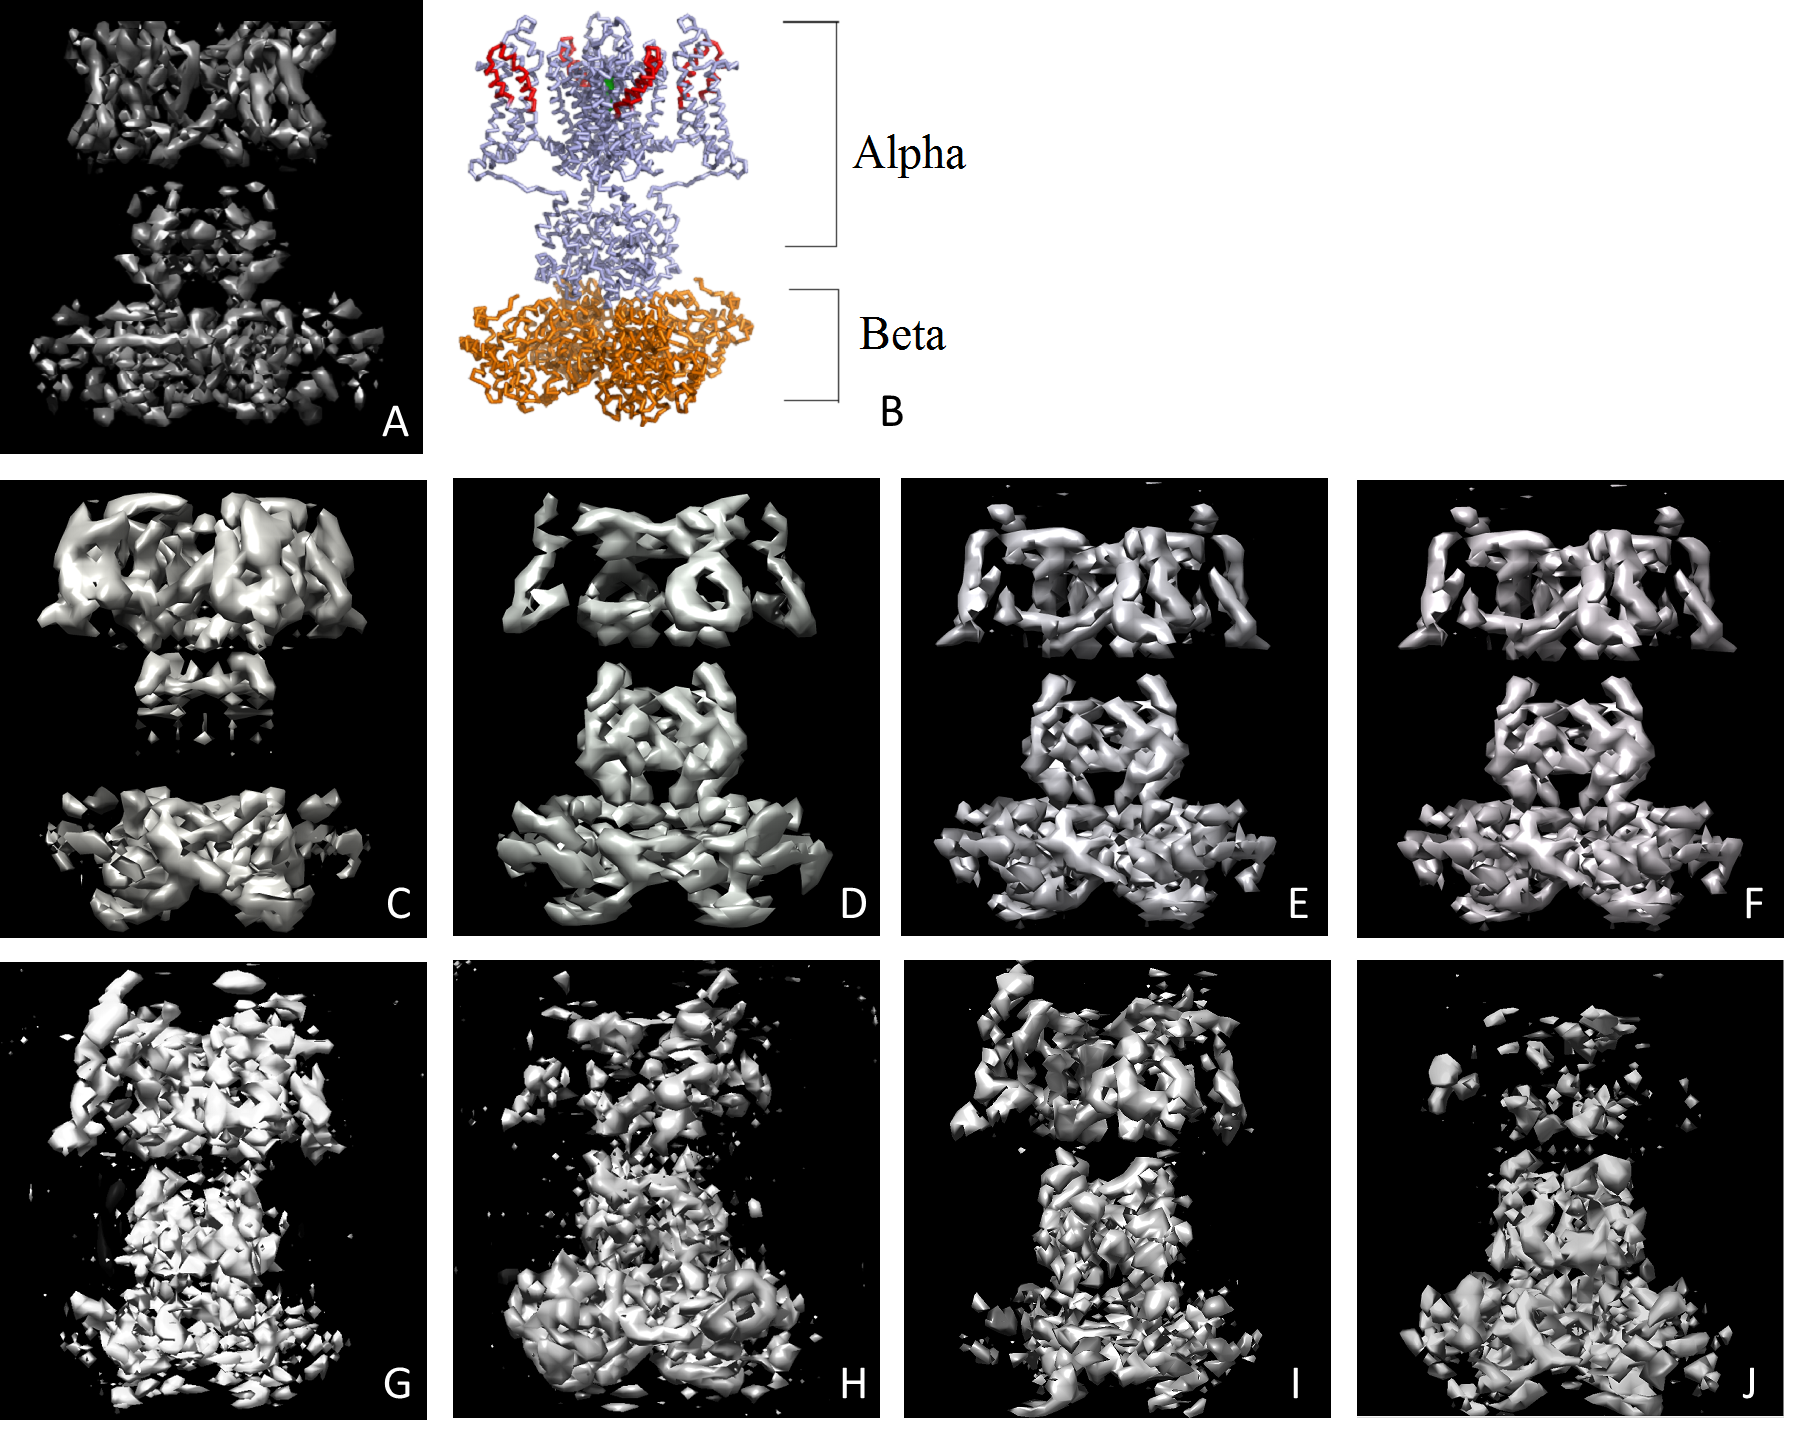
\includegraphics[width=.99\columnwidth]{reconstruction_all.png}
\end{center}
\vspace{-.1in}
\caption{Kv1.2 potassium channel: A) Volume visualization in UCSF Chimera \cite{chimera}. B) Image from Protein Data Bank Japan (PDBj). C through F show reconstructions from clean images - C) OE with $\alpha_4$ known, D) OE with $\beta_4$ known, E) OR with $\alpha_4$ known, and F) OE with $\beta_4$ known. G through J show reconstructions from noisy images using OR - G) SNR=0.7 with $\alpha_4$ known, H) SNR=0.7 with $\beta_4$ known, I) SNR=0.35 with $\alpha_4$ known, and J) SNR=0.35 with $\beta_4$ known.}
\label{fig:truth}
\vspace{-.1in}
\end{figure}
\subsubsection{Exact Recovery}
For OR, we have theoretical guarantee on recovery of the $O_l^{(1)}$ and $O_l^{(2)}$ as follows.
\begin{thm}\label{thm:recovery}
Assume that $A_l^{(1)}$ and $A_l^{(2)}\in\mathbb{R}^{K\times (2l+1)}$ are elementwise sampled from i.i.d. Gaussian $N(0,1)$, and $K>2l+1$, then the SDP method recovers $O_l^{(1)}$ and $O_l^{(2)}$ with probability $1$.
\end{thm}

The proof of Theorem~\ref{thm:recovery} is rather involved and we will put it in a separate work (Amit, what is the plan??- Teng) We remark that Theorem~\ref{thm:recovery} also holds if $A_l^{(i)}$ are complex-valued and $O_l^{(i)}$ are unitary matrices. Theorem~\ref{thm:recovery} shows that the power of the SDP method is close to the theoretical information limit since by counting the degrees of theorem, it is impossible to recover $O_l^{(1)}$ and $O_l^{(2)}$ if $K< 2l$.

\subsection{Resolution Limit}
(\ref{lin}) is a system of linear equations for $O_l^{(1)}$ and $O_l^{(2)}$
which can be estimated using least squares.
The number of free parameters associated with an orthogonal matrix in
$O(2l+1)$ is $l(2l+1)$. But the least squares
method does not constrain $O_l^{(1)}$ and $O_l^{(2)}$ to $O(2l+1)$.
Instead the solutions can be any
square matrices of size $2l+1$. So the effective total number of
variables for the least squares problem
is $2(2l+1)^2$. The number of linear equations in (\ref{lin}) is $K(2l+1)$.
Thus, using least squares we can resolve a truncated
spherical harmonic expansion
for $\phi^{(1)}$ and $\phi^{(2)}$ only for angular frequencies $l$ that satisfy
$K(2l+1) \geq 2(2l+1)^2$, that is, $l \leq \frac{K}{4} - \frac{1}{2}$.
This introduces a natural resolution limit on structures that can be resolved.
Ideally, we would like the least squares solution to take values in the orthogonal
group since this would impose a less strict resolution
limit on structures resolved, given by $l \leq \frac{K}{2}$. Thus, we see
that OR has the advantage of having an improved resolution limit.

\section{Numerical experiments}

We present the results of numerical experiments on simulated images ($109\times 109$ pixels) of the Kv1.2 potassium
channel complex (Fig.~\ref{fig:truth} A and B) and reconstruct its structure from clean and noisy
projection images. The experiments were performed in MATLAB in UNIX environment on an
Intel (R) Xeon(R) X7542 with 2 CPUs, having 6 cores each, running at 2.67 GHz, and with
256 GB RAM in total. 

Kv1.2 is a dumbbell-shaped particle consisting of two subunits - a small $\beta_4$ subunit
and a larger $\alpha_4$ subunit, connected by a central connector. We performed
experiments using OE and OR, assuming one of the subunits, for e.g. $\alpha_4$,  is known
while the other, $\beta_4$, is unknown. In the case of OR, we additionally use projection
images of the unknown subunit. 


%The images are of size $109 \times 109$. We experiments using OE: (i) Assuming
%the $\beta_4$ complex is known and (ii) the $\alpha_4$ complex is known. Despite the small size of
%$\beta_4$, we obtained a decent reconstruction in case (i). For OR also we perform two
%kinds of experiments: (i) $\beta_4$ is known and in addition also use the information in
%the projection images of the $\alpha_4$ complex alone and (ii) $\alpha_4$ is known and in
%addition also use the information inthe projection images of the $\beta_4$ complex alone .

%\begin{figure}[t]
%\begin{center}
%\includegraphics[width=.24\columnwidth]{cat_alpha.png} \includegraphics[width=.24\columnwidth]{cat_beta.png} \includegraphics[width=.24\columnwidth]{sdpalpha.png} \includegraphics[width=.24\columnwidth]{sdpbeta.png}
%\end{center}
%\caption{Reconstructions from clean images. Leftmost: OE with $\alpha_4$ known. Middle left: OE with $\beta_4$ known. Middle right: OR with $\alpha_4$ known. Rightmost: OE with $\beta_4$ knowvn}
%\label{fig:clean}
%%\vspace{-.35in}
%\end{figure}
%\vspace{-.15in}

\begin{figure}[b]
\centering
  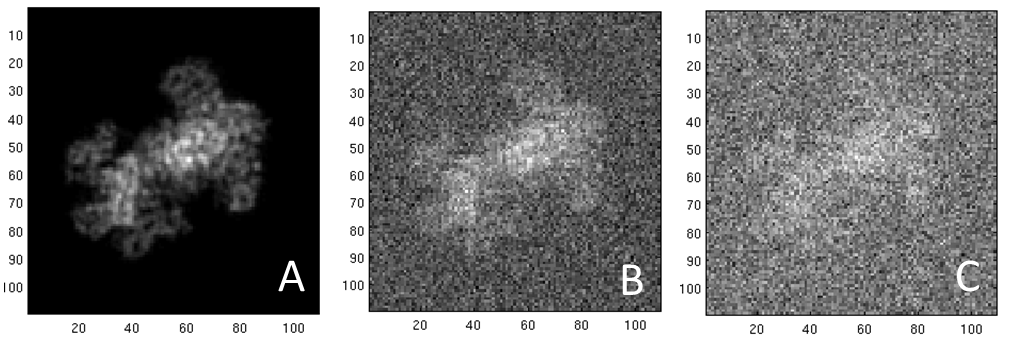
\includegraphics[width=.9\columnwidth]{proj_all.png}
  \caption{Projection images at different values of SNR: A) Clean image, B) SNR=0.7, and
  C) SNR=0.35.}
\label{fig:proj}
\end{figure}
\vspace{-.15in}


%\begin{figure}[t]
%\begin{center}
%\includegraphics[width=.24\columnwidth]{noise07alpha.png} \includegraphics[width=.24\columnwidth]{noise07beta.png} \includegraphics[width=.24\columnwidth]{noise035alpha.png} \includegraphics[width=.24\columnwidth]{noise035beta.png}
%%\includegraphics[width=.49\columnwidth]{noise035alpha.png} \includegraphics[width=.49\columnwidth]{noise035alpha.png}
%\end{center}
%\caption{Reconstruction from noisy images using OR. Leftmost: SNR=0.7 with $\alpha_4$ known. Middle left: SNR=0.7 with $\beta_4$ known. Middle right: SNR=0.35 with $\alpha_4$ known. Rightmost: SNR=0.35 with $\beta_4$ known}
%\label{fig:noisy}
%%\vspace{-.35in}
%\end{figure}
%\vspace{-.15in}

\subsection{Clean and Noisy Projections}
We reconstruct the structure from both clean and noisy projection images. The
reconstruction of Kv1.2 obtained from clean images using OE and OR is shown in
Fig.~\ref{fig:truth} C through F. We used the true $C_l$ matrices for the known subunit, and a maximum
$l$ of 30. We tested OR to reconstruct Kv1.2 from noisy projections at various values of
SNR. A sample projection image at different values of SNR is shown in Fig.~\ref{fig:proj}.
The $C_l$ matrices were estimated from the noisy projection images. In
Fig.~\ref{fig:truth} G through J we show the reconstructions obtained from 10000 projections using OR
at SNR=0.7, and from 40000 projections using OR at SNR=0.35.

\subsection{Comparison between OE and OR}
We quantify the `goodness' of the reconstruction using the Fourier Cross Resolution (FCR)
\cite{fcr}. FCR measures the normalized cross correlation between two 3D volumes over
corresponding spherical shells in Fourier space - first, the reconstruction from noisy
images, and second, the ground truth. In Fig. \ref{fig:fsc} we show the FCR curves for the
reconstruction from the $\beta_4$ complex using OE and OR. The additional information in
OR, from the projection images of $\alpha_4$, results in a better reconstruction, as seen
from the FCR curve. The Kv1.2 complex has $C4$ symmetry, which reduces the rank of the
$C_l$ matrices. Our experiment thus benefits from the reduced size of the orthogonal
matrices to be recovered.

\begin{figure}[t]
  \centering
  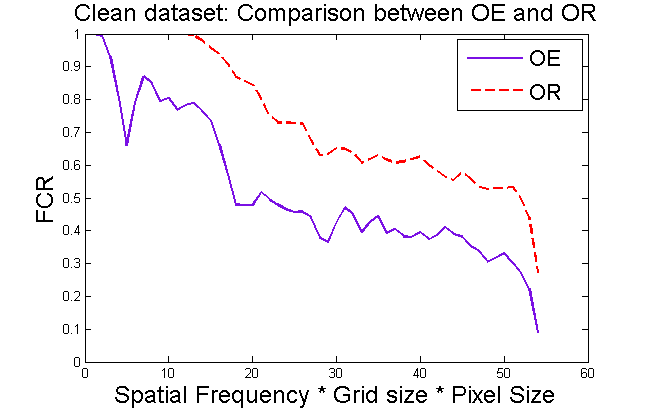
\includegraphics[width=.7\columnwidth]{FSC_final.png}
  \caption{FCR curve for reconstruction from $\beta_4$ (clean images)}\label{fig:fsc}
\end{figure}
\vspace{-.15in}
\subsection{Computational Complexity}
The OE method requires the Cholesky decomposition of $C_l$ and the SVD of $\tilde{A_l^\star}F_l$, which has a computational complexity of $O(K^3)$.
The OR method requires solving a SDP problem of size $3(2l+1)\times 3(2l+1)$ with $3(l+1)(2l+1)$ linear constraints, and the theoretical running time of the interior point method is $O(l^{6.5})$~\cite[Section 4.6.3]{ben2001lectures}. In practice we use the MATLAB package CVX to solve the SDP. In our simulation with 10000 images, it took $416.36$ seconds to perform steerable PCA and $194.04$ seconds to calculate the $C_l$ matrices (using the maximum $l$ as 30). The running time to solve the SDP as a function of $l$ is recorded in Table~\ref{table:timing}.
\begin{table}[h!]
\vspace{-.05in}
\begin{center}
\begin{tabular}{|c|c|}
\hline
$l$  & Time (seconds)  \\
\hline
5 & 5.71  \\
\hline
10 & 18.95 \\
\hline
15 & 50.69 \\
\hline
20 & 108.61  \\
\hline
25 & 163.20  \\
\hline
30 & 193.76   \\
\hline
\end{tabular}
\end{center}
\vspace{-.1in}
\caption{Timing (in seconds) to solve the SDP with the MATLAB CVX package.}
\label{table:timing}
\end{table}
\vspace{-.15in}
\section{Conclusion}
Reconstruction of small complexes is a long-standing problem in cryo-EM that poses a limit on its applicability.
We expect the methods described in this paper to enhance the capabilities of three-dimensional electron microscopy techniques
and be able to answer biological questions related to small protein structures that have so far remained unresolved.
In the future, we plan to characterize the performance of these
algorithms and their accuracy as a function of the number of images, the SNR, and the resolution, and test these methods on real datasets.


% References should be produced using the bibtex program from suitable
% BiBTeX files (here: strings, refs, manuals). The IEEEbib.bst bibliography
% style file from IEEE produces unsorted bibliography list.
% -------------------------------------------------------------------------
\bibliographystyle{IEEEbib}
\bibliography{ur_draft1}


\end{document}

% \begin{figure}
% \centering
% \begin{subfigure}{.25\textwidth}
%   \centering
%   \includegraphics[width=.7\linewidth]{noise07alpha.png}
%   \caption{OR: $\alpha_4$ known}\label{fig:noisealpha}
%   \label{fig:sub1}
% \end{subfigure}%
% \begin{subfigure}{.25\textwidth}
%   \centering
%   \includegraphics[width=.7\linewidth]{noise07beta.png}
%   \caption{OR: $\beta_4$ known}\label{fig:noisebeta}
%   \label{fig:sub2}
% \end{subfigure}
% \caption{Reconstruction from noisy images. SNR=0.7}
% \label{fig:noisy}
% \end{figure}
% \begin{figure}
% \centering
% \begin{subfigure}{.25\textwidth}
%   \centering
%   \includegraphics[width=.7\linewidth]{noise035alpha.png}
%   \caption{OR: $\alpha_4$ known}\label{fig:noisealpha035}
%   \label{fig:sub1}
% \end{subfigure}%
% \begin{subfigure}{.25\textwidth}
%   \centering
%   \includegraphics[width=.7\linewidth]{noise035beta.png}
%   \caption{OR: $\beta_4$ known}\label{fig:noisebeta035}
%   \label{fig:sub2}
% \end{subfigure}
% \caption{Reconstruction from noisy images. SNR=0.35}
% \label{fig:noisy035}
% \end{figure}
% \begin{figure}
% \centering
% \begin{minipage}{.2\textwidth}
%   \centering
%   \includegraphics[width=.5\linewidth]{noise07alpha.png}
%   \caption{OR: $\alpha_4$ known}\label{fig:noisealpha}
%   \label{fig:test1}
% \end{minipage}%
% \begin{minipage}{.2\textwidth}
%   \centering
%   \includegraphics[width=.5\linewidth]{noise07beta.png}
%   \caption{OR: $\beta_4$ known}\label{fig:noisebeta}
%   \label{fig:test2}
% \end{minipage}
% \end{figure}


% \includegraphics[width=.49\columnwidth]{cat_alpha.png} \includegraphics[width=.49\columnwidth]{cat_beta}
% \begin{figure}
% \centering
% \begin{subfigure}{.25\textwidth}
%   \centering
%   \includegraphics[width=.49\columnwidth]{cat_alpha.png} \includegraphics[width=.49\columnwidth]{cat_beta}
%   \caption{Reconstruction from clean images. Top left: OE with $\alpha_4$ known. Top right: OE with $\beta_4$ known}
%   \label{fig:sub1}
% \end{subfigure}%
% \begin{subfigure}{.25\textwidth}
%   \centering
%   \includegraphics[width=.7\linewidth]{cat_beta.png}
%   \caption{OE: $\beta_4$ known}\label{fig:catbeta}
%   \label{fig:sub2}
% \end{subfigure}
% \caption{Reconstruction from clean images using OE}
% \label{fig:cleanOE}
% \end{figure}
% \begin{figure}
% \centering
% \begin{subfigure}{.25\textwidth}
%   \centering
%   \includegraphics[width=.7\linewidth]{sdpalpha.png}
%   \caption{OR: $\alpha_4$ known}\label{fig:sdpalpha}
%   \label{fig:sub1}
% \end{subfigure}%
% \begin{subfigure}{.25\textwidth}
%   \centering
%   \includegraphics[width=.7\linewidth]{sdpbeta.png}
%   \caption{OR: $\beta_4$ known}\label{fig:sdpbeta}
%   \label{fig:sub2}
% \end{subfigure}
% \caption{Reconstruction from clean images using OR}
% \label{fig:cleanOR}
% \end{figure}


% \begin{figure}
% \centering
% \begin{subfigure}{.25\textwidth}
%   \centering
%   \includegraphics[width=.7\linewidth]{truth.png}
%   \caption{}
%   \label{fig:kvtrue}
% \end{subfigure}%
% \begin{subfigure}{.25\textwidth}
%   \centering
%   \includegraphics[width=.7\linewidth]{kv12.PNG}
%   \caption{}
%   \label{fig:kvscheme}
% \end{subfigure}
% \caption{Kv1.2 potassium channel}
% \label{fig:truth}
% \end{figure}
% \begin{figure}
% \centering
% \begin{minipage}{.2\textwidth}
%   \centering
%   \includegraphics[width=.5\linewidth]{cat_alpha.png}
%   \caption{OE: $\alpha_4$ known}\label{fig:catalpha}
%   \label{fig:test1}
% \end{minipage}%
% \begin{minipage}{.2\textwidth}
%   \centering
%   \includegraphics[width=.5\linewidth]{cat_beta.png}
%   \caption{OE: $\beta_4$ known}\label{fig:catbeta}
%   \label{fig:test2}
% \end{minipage}
% \end{figure}

%  One approach to solve
% (\ref{noncon}) is to use an alternating least squares (ALS) procedure, which is
% an iterative procedure that alternates
% between updating $O_l^{(1)}$ and $O_l^{(2)}$.
% \begin{equation*}\label{noncon}
% O_l^{(1)} \leftarrow \argmin_{O_l^{(1)} \in O(2l+1)}
% ||F_l^{(2)}-F_l^{(1)}-G_l^{(2)}O_l^{(2)}-G_l^{(1)}O_l^{(1)} ||_F^2
% \end{equation*}
% \begin{equation}\label{noncon}
% O_l^{(2)} \leftarrow \argmin_{O_l^{(1)} \in O(2l+1)}
% ||F_l^{(2)}-F_l^{(1)}-G_l^{(2)}O_l^{(2)}-G_l^{(1)}O_l^{(1)} ||_F^2
% \end{equation}
% These update rules have a closed form solution using singular value
% decomposition. Each iteration reduces the value of
% the cost function in (\ref{noncon}), so the iterates converge to a local but non
% necessarily global minimum. Numerical
% simulations show that ALS does not converge to a global minimum unless we start
% with a good initialization. 
